\chapter{Analysis of the Data\label{cha:chapter4}}
%This chapter introduces the architectural design of Component X. The component consists of subcomponent A, B and C.

%In the end of this chapter you should write a specification for your solution, including interfaces, protocols and parameters.
Idealo has organised its products into a tree structure of categories. Each product is classified into a category. That is, having a set of target categories $C = {c_1, c_2, ..., c_t}$ and a set of products $P = {p_1, p_2, ..., p_n}$:

\begin{center}
    $(\forall p_i \in P, \exists c_j \in C : l(p_i) = c_j $)  \\
\end{center}

Where $l$ is function that maps a product to a category, such that:\\

\begin{center}
    $l: P \rightarrow C$. \label{eq:classifierFunction}\\
\end{center}

Categories are arranged in a human-elaborated tree structure, where categories in the upper levels of the tree are related to more general definitions (e.g. Telecommunications, Computer\&Hardware, Fashion\&Accessories...), and leaves or categories in deeper levels represents more specific categories (e.g: Red Wines, Bank Benches, Footballs...).For example, \textit{Pictonary} is a famous and nice board game, this is how it looks part of its page at idealo's website (see figure \ref{fig:pictionary})

\begin{figure}[!htbp]
  \centering
  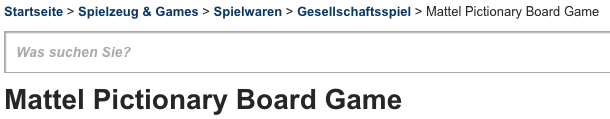
\includegraphics[width=10cm]{pictionary.png}\\
  \caption{Path of categories for a product}
  \label{fig:pictionary}
\end{figure}

\textit{Pictonary} is classified as a \textit{Gesellschaftsspiel} (board game). It's important to notice, that we can see already in the interface of the website that this category has \textit{Spielwaren} (toys) as its parent in the category tree, and the latter is a child of the \textit{Spielzeug\&Games} (toys and games) category, which is a first level category (\textit{Startseite} is the root).

Notice that products can belong to any category in the tree (i.e. classification is not exclusive into leaf categories, but also node categories). Figure \ref{fig:idealoTree} shows a general overview of the structure of the category tree.

\begin{figure}[!htbp]
  \centering
  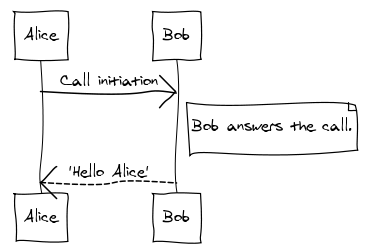
\includegraphics[width=9cm]{uml_seq_example.png}\\
  \caption{Category Tree}
  \label{fig:idealoTree}
\end{figure}


\section{Where does the Classifier fit?\label{sec:classifier}}
%Explain where is situated the classifier in the Idealo's structure or the path of an offer.
The route a product follows since it is retrieved from an online-shop till it is showed to the final user in the website is a long path. After a product is retrieved, it's determined whether it's a new product or something that has been seen before by trusted classification processes. Also, a set of rules are employed to reduce the amount of products that need to be classified (knowledge engineering). Then, after some products are already out, X\% makes it to the classifier that uses machine learning techniques. 
For the classifier's decision to be taken into account, it needs to have 80\% of confidence in the answer it's giving.
Products that aren't classified by any of this stages are manually classified by domain experts (i.e. items that had less than 80\% of confidence in the classifier).

The classifier is a supervised learning algorithm that assigns a unique label (category) to every given datapoint (product) (See equation ~\ref{eq:classifierFunction}). From now on, we will assume we are only inside the classifier context (i.e. products and categories are those that the classifier knows).

\section{The Categories \label{sec:conceptsubb}}

%Structure of the categories, the taxonomy, distributions, etc.
All categories are structured into a category tree that was built by domain experts. Nodes and leaves from the tree are categories that may be target-categories. 
When a product is assigned to one target-category, it means that this product also (implicitly) belongs to all the categories that conform the path from this (target-)category up to the root of the tree. For example, given the subtree in figure \ref{fig:subtree}, a product that was assigned to be in the \textit{Art} target-category, would be implicitly  belong to \textit{Culture} and \textit{Encyclopedia} (root) too.

\begin{figure}[!htbp]
  \centering
  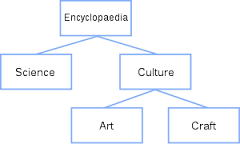
\includegraphics[width=9cm]{treeEx.png}\\
  \caption{SubTree}
  \label{fig:subtree}
\end{figure}

As said before, products aren't exclusively classified into leaf categories (i.e. node-categories are sometimes subject of classification too). Let's say we have an Encyclopedia for Cultural Expressions. This product fits exactly in the \textit{Culture} category, therefore this product should be classified as \textit{Culture}. Nevertheless this is implicitly also classified as \textit{Encyclopedia}, as it's parent of the target-category \textit{Culture}. 

Now that we have understood intuitively this concepts, let's built a mathematical definition out of it. Let $C$ be a set containing all categories, $C = {c_1, c_2, ..., c_t}$ and $P$ the set of products $P = {p_1, p_2, ..., p_n}$. Let $R = {r_1, r_2..., r_t}$ be a set that contains the root paths of all categories in $C$, that is $r_i \subseteq C$ is a set that contains the path from the root of the tree to the node/leaf $c_i$. Then, when a product $p_j$ is classified as $c_i$ ($l(p_j) = c_i$), implicitly, $p_j$ also belongs to all categories in $r_i$.

Then, the classifier ($l: P \rightarrow C$) should select the target-category that first suites better a product, and second its located in the highest level of the tree of categories (i.e. the most suitable deepest category in the tree).

\subsection{The Taxonomy}
%explain the taxonomy, the fact that a category can be a node AND a category subject of classification (not only leaves).
The Categories' taxonomy is a very wide tree with 6 levels. It presents a very uneven distribution of the categories among its branches (see figure \ref{fig:distCats}). As seen in table \ref{tab:categoryDist}, the first level of the tree contains 13 categories. All of this 13 categories (there are 0 leaves at this level), have in average 11 children. The first-level category with less children contains 8, and the one with most have 16. X out of 13 are target categories in the first category (i.e. products are classified into those).
In the last level of the tree, there's only 4 leaf-categories.

\begin{figure}[!htbp]
  \centering
  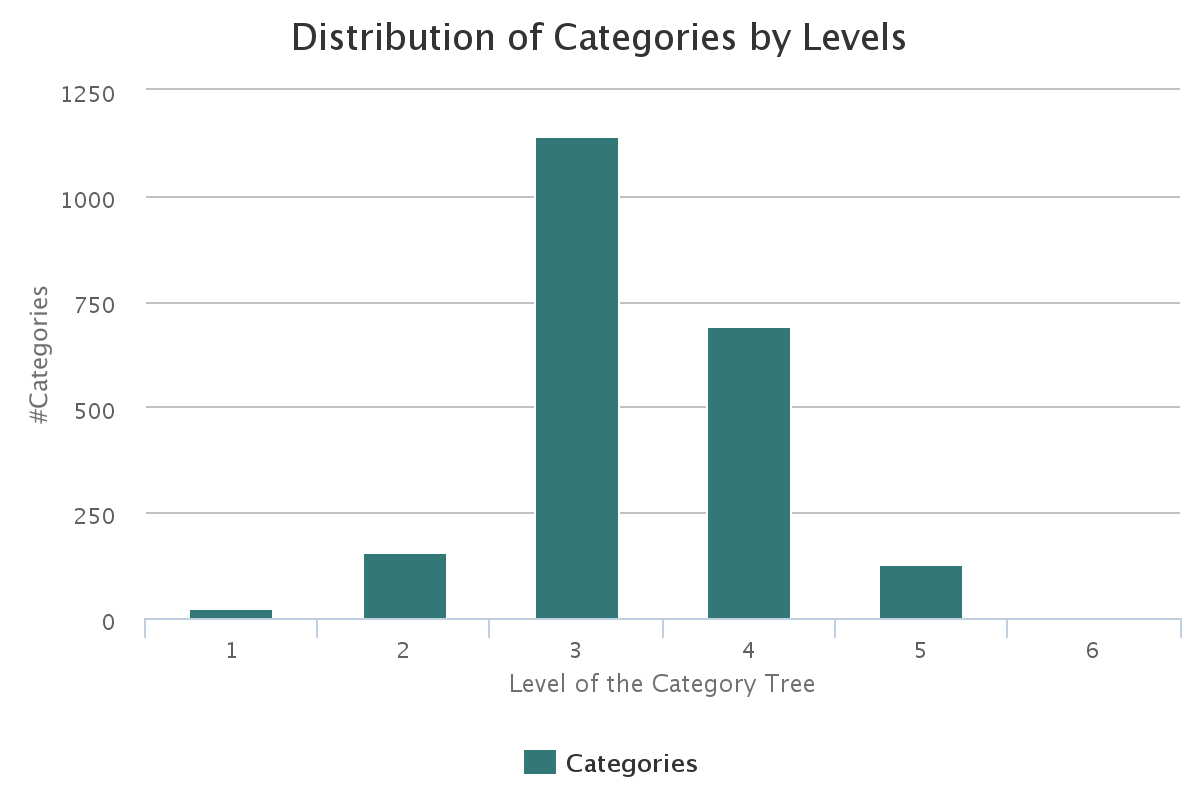
\includegraphics[width=14cm]{DistCatsLevels.png}\\
  \caption{Distribution of Categories across levels of the category tree}
  \label{fig:distCats}
\end{figure}

\begin{table}[!htbp]
    \centering
    \begin{tabular}{|c|c| C{1.5cm} | C{1.5cm} | C{1.5cm}| C{1.5cm}|C{1.5cm}|}
       \hline
       Level &  X-Level & \multicolumn{5}{c|}{Category Node Withing Level-X Nodes} \\
       \cline{3-7}
         & Categories & Avg & Min & Max & Leaves & Target  \\
       \hline
        1 & 13 & 11 & 8 & 16 & 0 & \\
        2 & 152 & 11 & 47 &1 & 52 & \\
        3 & 1138 & 8 & 46 & 1 & 1056&  \\
        4 & 686 & 6 & 12 & 2 & 663& \\
        5 & 128 & 4 & 4 & 4 & 127& \\
        6 & 4 & 0 & 0 & 0 & 4 & 4 \\
        \hline
        
    \end{tabular}
    \caption{Distribution of Categories in the Category Tree}
    \label{tab:categoryDist}
\end{table}


\section{The Products\label{sec:conceptsubb}}

%Structure of Angebote, relation with categories
Products have several features that can be used for the classification task. The main problem about this, is that it consists of a very heterogenuos representation: not always all features exist in all products.
From all existent features, this are the one that were chosen for this project
\begin{itemize}
    \item Title: this is one of the features that products lack the less. It's the title of a product that is retrieved from the retailers. It's a text field, that on average has 11 words.
    \item Description: this text field describe or explain what the product is.
    \item Brand: the brand of the product
    \item Attributes: a list of attributes that a product has (such as size, in the case of shoes, RAM in the case of computers, etc.). There are up to 8005 different alternatives for attributes.
    \item productSearchText:
    \item shopKategorie:
\end{itemize}

From the uneven distribution of categories across levels in the tree, it's already expected that the products are also unevenly distributed across levels in the tree. This is confirmed in figure \ref{fig:productsDist}
\begin{figure}[!htbp]
  \centering
  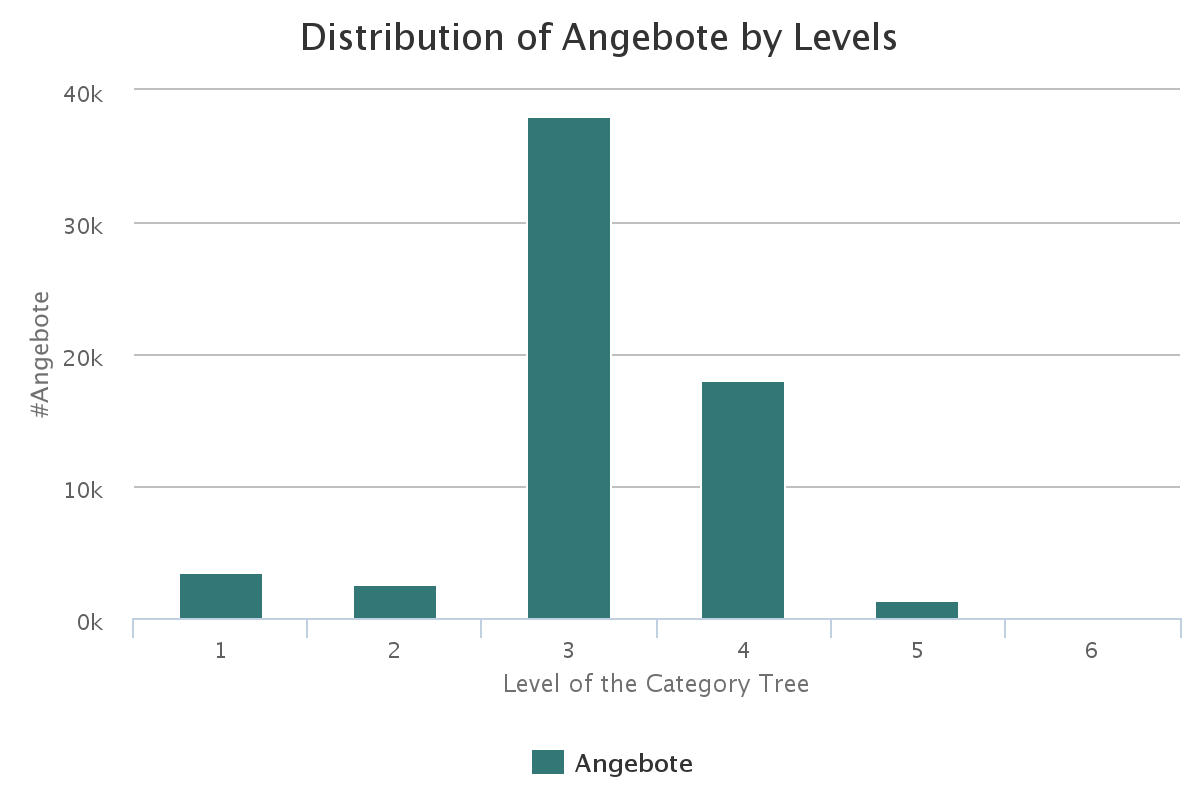
\includegraphics[width=14cm]{DistAngeLevels.png}\\
  \caption{Distribution of Products across levels of the category tree}
  \label{fig:productsDist}
\end{figure}

This uneven distribution is not just across levels in the tree, also includes the outdegree of categories (see figure \ref{fig:distProdCats})

\begin{figure}[!htbp]
  \centering
  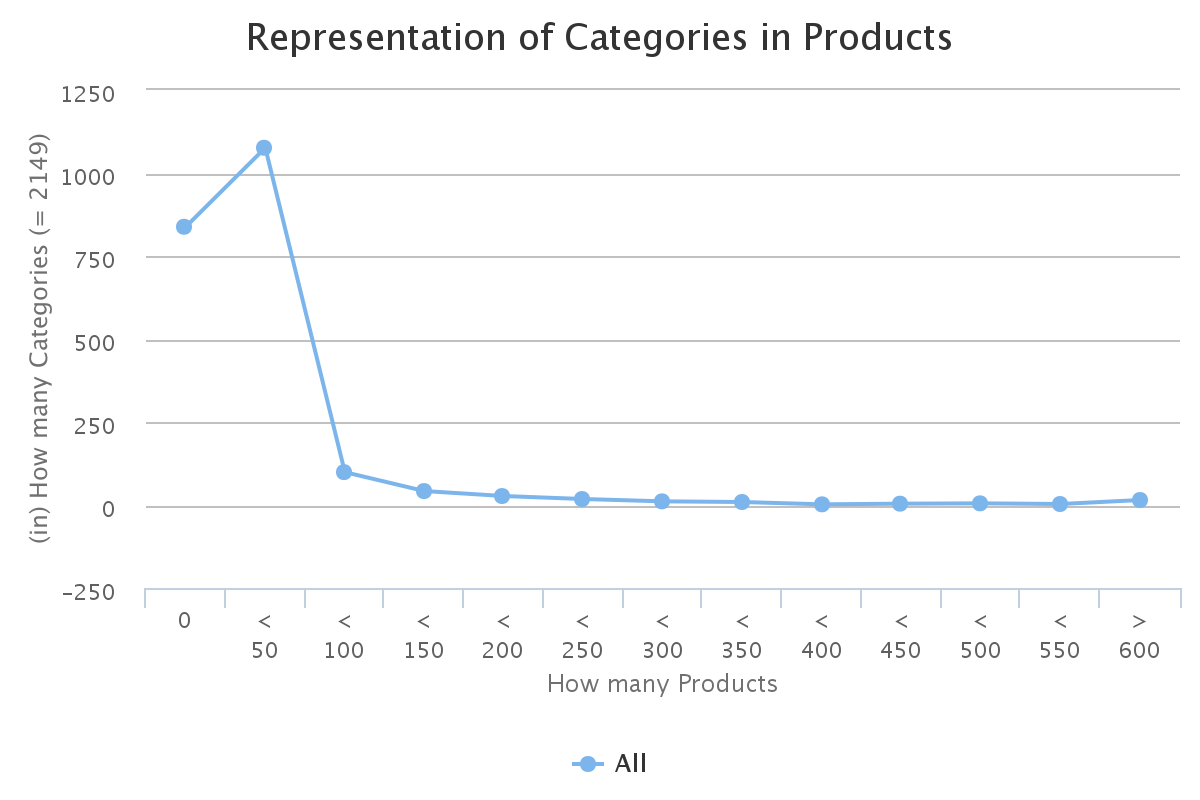
\includegraphics[width=14cm]{DistProductsOverCats2.png}\\
  \caption{Distribution of Products over Categories}
  \label{fig:distProdCats}
\end{figure}

\section{Problems with the Data\label{sec:conceptlayerx}}
Natural language problems: misspelling, german umlaut. 
Not balanced Data: Distribution... (pic)
Irregularities in Data: other alphabet (japanesse, corean...), IDs,

Uneven distribution, LinkedTarget, empty features, ghost categories, lack of quality for some classified products (misclassified in training data)...EXAMPLES!. 

Classification of misspelled stuff

\section{The Classification Task}
General explanation based on the showed plots, how will be classified the data (e.g. coarse-grained approach), play with features at each level.

\section{Place of Work\label{sec:conceptinter}}

Cluster, PC, etc (memory, OS, processors, etc)

\section{Spark with Scala\label{sec:intspec}}

Lorem Ipsum...

